\section{Moulinette}
\label{sec::moulinette}

\begin{figure}[H]
	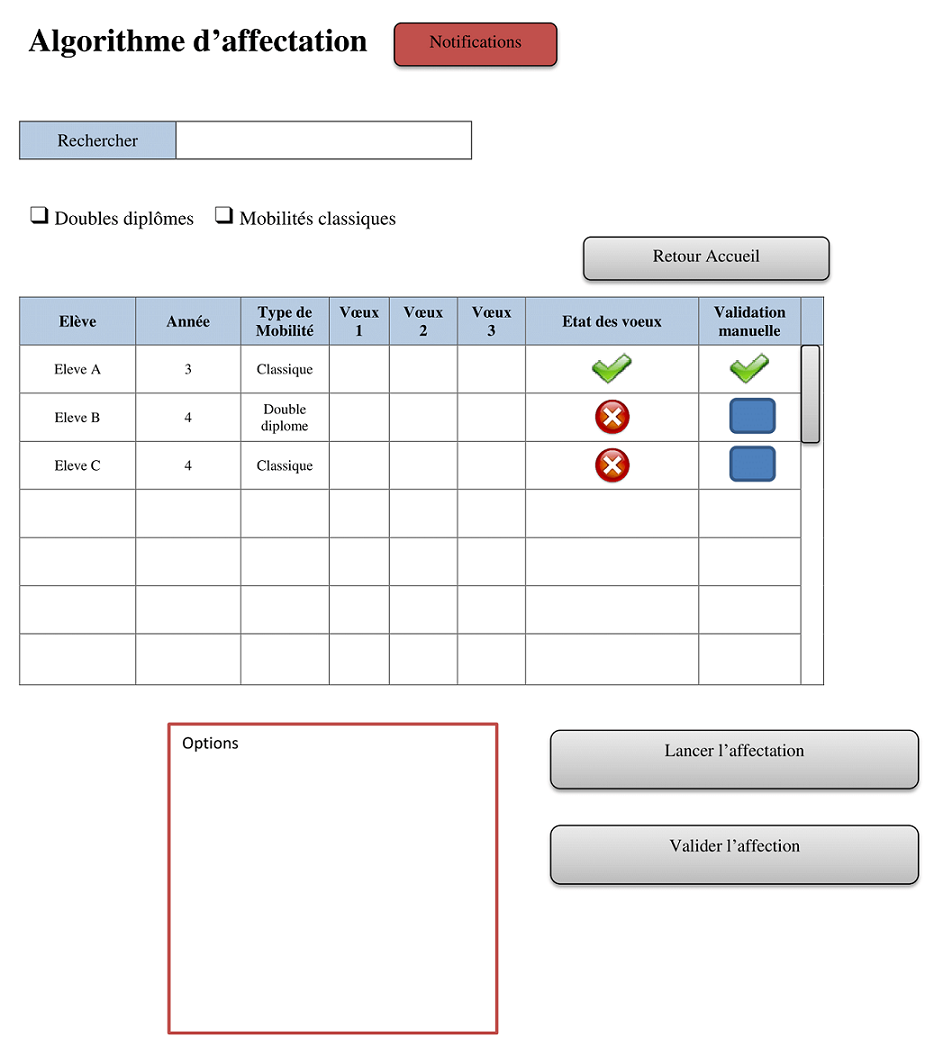
\includegraphics[scale=0.7]{Admin/Moul.png}
	\caption{Page de gestion de la moulinette}
\end{figure}

Sur cette page ce trouve un tableau récapitulant les vœux définitif des élèves après la fin des choix de vœux (phase 1). Ce tableau comprend donc la liste des élèves, leur année, la liste des vœux, le type de mobilité choisie (double diplôme, mobilité classique), leur état (validé, à validé).
Encore présent sur ce tableau; une zone de recherche par mot clé ainsi que plusieurs filtres (années, universités, type de mobilité...).\\

L'administrateur peut, sur cette page, gérer les paramètres de la moulinette avant de la lancer (ajout de paramètres particuliers modifiant l'ordre d'attribution des vœux en plus des notes).\\

Il est aussi possible à l'administrateur de validé les vœux d'un élève manuellement. Cela fait sortir cet élève de la liste des élèves concernés par la moulinette (il apparaitra toujours dans la liste des élèves mais son état deviendra "validé" et il sera pas pris en compte par la moulinette).\\

Enfin, un bouton permettant de lancer l'algorithme d'attribution des vœux. Lorsque que l'algorithme est terminé la phase 1 est terminée et la phase 2 est lancée. Cela signifie que les différentes vue deviendrons celles de la phase 2.